\documentclass[titlepage]{article}
\usepackage[utf8x]{inputenc}
\usepackage[english]{babel}
\usepackage{amsmath}
\usepackage{float}
\usepackage{pgfplots}
\usepackage[left=1.5in, right=1.0in, top=1.0in, bottom=1.0in, a4paper]{geometry}
\usepackage{listings}
\usepackage{lmodern}
\usepackage{fancyhdr}
\usepackage{enumitem}
\usepackage{hyperref}
\usepackage{xcolor}
\usepackage{authblk}

\pagestyle{fancy}
\fancyhf{}
\fancyfoot[R]{\thepage}

%----------------------------------------------------------------------------------------
%	Code block styles
%----------------------------------------------------------------------------------------

\definecolor{comment}{RGB}{0,128,0} % dark green

\lstdefinestyle{c}{
	commentstyle=\color{comment},
    keywordstyle=\color{blue},
	basicstyle=\footnotesize\ttfamily,
	frame=single,
	breaklines=true,
	showstringspaces=false,
	upquote=true,
	tabsize=2
}
\lstdefinestyle{inlineC}{
	basicstyle=\footnotesize\ttfamily,
	breaklines=true,
	showstringspaces=false,
	upquote=true,
	tabsize=2
}

%----------------------------------------------------------------------------------------
%	Variables section
%----------------------------------------------------------------------------------------

\title{\textbf{Assignment 2: Solving the Heat Equation using
several Parallel Programming Models} \\
[0.2in]
CPDS: Parallelism
}

\author[*]{Edgar Rodriguez De La Calle}
\author[*]{Nicolás Zhao}
\affil[*]{Universitat Politècnica de Catalunya}
\affil[ ]{\textit {cpds\{1122,1104\}}}
\affil[ ]{\textit {\{edgar.rodriguez.de.la.calle,nicolas.zhao\}@estudiantat.upc.edu}}

\date{\today}

\renewcommand{\headrulewidth}{0pt} % Remove header underlines
\renewcommand{\footrulewidth}{0pt} % Remove fooQter underlines
\newcommand{\incode}[1]{\lstinline[style=inlineC,language=C]{#1}}
\renewcommand{\lstlistingname}{Code}%

\newcounter{qcounter}
\setcounter{qcounter}{0}
\newcounter{subqcounter}[qcounter]

% Define custom command for questions
\newcommand{\q}[1]{%
    \stepcounter{qcounter} % Increment question number
    \setcounter{subqcounter}{0} % Reset subquestion counter for new question
    \section{Problem \arabic{qcounter}}
        #1
    \medskip
}
\newcommand{\subq}[1]{
    \stepcounter{subqcounter} % Increment subquestion number
    \subsection{Problem \arabic{qcounter}.\arabic{subqcounter}}
    #1
    \medskip
}
\pgfplotsset{compat=1.18}

\begin{document}

\maketitle
\pagebreak

\setcounter{secnumdepth}{0}

\q{Explain briefly the parallelization of the heat equation application that you have done for each programming model (OpenMP, MPI and CUDA).}

\subsection{OpenMP}

\subsubsection{Jacobi}

For the Jacobi solver we have add \incode{#pragma omp parallel for reduction(+: sum) private(diff)} statement to the outer loop that is used to iterate between the blocks/tiles.

To allow the partition of workload between the threads we have also change the values of \incode{nbx}, \incode{nby}, \incode{bx} and \incode{by} to take \incode{OMP_NUM_THREADS} into account.

\begin{lstlisting}[style=c, language=C, caption=OpenMP Jacobi, captionpos=b]      
double relax_jacobi (double *u, double *utmp, unsigned sizex, unsigned sizey)
{
    double diff, sum=0.0;

    #pragma omp parallel for collapse(2) private(diff) reduction(+: sum) 
    for (unsigned int i = 1; i < sizex-1; i++) 
        for (unsigned int j = 1; j < sizey-1; j++) {
            utmp[i*sizey+j]= 0.25 * (u[ i*sizey + (j-1)] +  // left
                    u[i*sizey + (j+1)] +  // right
                    u[(i-1)*sizey + j] +  // top
                    u[(i+1)*sizey + j]);  // bottom
            diff = utmp[i*sizey+j] - u[i*sizey + j];
            sum += diff * diff; 
        }

    return sum;
}

\end{lstlisting}

\subsubsection{Gauss-Seidel}

For a tiled implementation of Gauss-Seidel we have changed the values of \incode{nbx}, \incode{nby}, \incode{bx} and \incode{by} to use \incode{OMP_NUM_THREADS} for split the data into tiles. For an in-depth explanation of Gauss-Seidel parallelization checkout Section \nameref{sec:mpi_gauss_seidel} (MPI)

\begin{lstlisting}[style=c, language=C, caption=OpenMP Tiled Gauss-Seidel, captionpos=b]      
nbx =  omp_get_max_threads();                        
bx = sizex/nbx;                                      
nby = omp_get_max_threads();                         
by = sizey/nby;
\end{lstlisting}

We have implemented 2 version of the \incode{relax_gauss} function:

\begin{itemize}
    \item Using explicit task dependence (\incode{relax_gauss_task})
    \item Using do-across (\incode{relax_gauss_ordered})
\end{itemize}

Explicit task dependence implementation has the following code:

\begin{lstlisting}[style=c, language=C, caption=OpenMP Gauss-Seidel with explicit task dependence, captionpos=b] 
double relax_gauss_task (double *u, unsigned sizex, unsigned sizey)
{
    double unew, diff, sum=0.0;
    int nbx, bx, nby, by;

    nbx = omp_get_max_threads(); 
    bx = sizex/nbx;
    nby = omp_get_max_threads(); 
    by = sizey/nby;

    int blocks[nbx][nby];

    #pragma omp parallel 
    #pragma omp single
    {
        for (int ii=0; ii<nbx; ii++){
            for (int jj=0; jj<nby; jj++) {
                #pragma omp task \
                        depend(in: blocks[ii-1][jj], blocks[ii][jj-1] ) \
                        depend(inout: blocks[ii][jj]) private(diff, unew) 
                {
                    double partial_sum = 0.0;
                    for (int i=1+ii*bx; i<=min((ii+1)*bx, sizex-2); i++){
                        for (int j=1+jj*by; j<=min((jj+1)*by, sizey-2); j++) {
                            unew= 0.25 * (    u[ i*sizey	+ (j-1) ]+  // left
                                    u[ i*sizey	+ (j+1) ]+  // right
                                    u[ (i-1)*sizey	+ j     ]+  // top
                                    u[ (i+1)*sizey	+ j     ]); // bottom
                            diff = unew - u[i*sizey+ j];
                            partial_sum += diff * diff; 
                            u[i*sizey+j]=unew;
                        }
                    }
                    #pragma omp atomic
                    sum += partial_sum;
                }
            }
        }
     }
    return sum;
}
\end{lstlisting}

Initially, we establish an auxiliary matrix called \incode{blocks} for specifying task dependencies in a subsequent step. We proceed by creating a parallel code segment using \incode{#pragma omp parallel}, followed by \incode{#pragma omp single} to ensure that only a single thread generates the tasks. Each task is responsible for computing the \incode{partial_sum} within a specific tile or block. To achieve this, we position the task directive within the two inner loops, which iterate through the values within each tile or block. Additionally, it's crucial to note that each task explicitly relies on neighboring tasks, a dependency we declare using \incode{depend(in: blocks[ii-1][jj], blocks[ii][jj-1]) depend(inout: blocks[ii][jj])}. This statement establishes a dependency for each task on its preceding task in the top and left positions. Lastly, we accumulate the \incode{partial_sum} from each task into the \incode{sum} variable. To prevent race conditions during this accumulation, we utilize \incode{#pragma omp atomic}.

Moving onto the do-across implementation, it has the following code:

\begin{lstlisting}[style=c, language=C, caption=Gauss-Seidel with do-across, captionpos=b] 
double relax_gauss_ordered (double *u, unsigned sizex, unsigned sizey)
{
    double unew, diff, sum=0.0;
    int nbx, bx, nby, by;

    nbx =  omp_get_max_threads();
    bx = sizex/nbx;
    nby = omp_get_max_threads(); 
    by = sizey/nby;

    #pragma omp parallel for collapse(2) ordered(2) reduction(+:sum) \
            private(diff, unew)
    for (int ii=0; ii<nbx; ii++){
        for (int jj=0; jj<nby; jj++){
            #pragma omp ordered depend(sink: ii-1, jj) depend(sink: ii,jj-1) 
            for (int i=1+ii*bx; i<=min((ii+1)*bx, sizex-2); i++){
                for (int j=1+jj*by; j<=min((jj+1)*by, sizey-2); j++) {
                    unew= 0.25 * (u[ i*sizey + (j-1) ]+  // left
                            u[i*sizey+(j+1) ]+  // right
                            u[(i-1)*sizey+ j]+  // top
                            u[(i+1)*sizey+ j]); // bottom
                    diff = unew - u[i*sizey+ j];
                    sum += diff * diff; 
                    u[i*sizey+j]=unew;
                }
            }
            #pragma omp ordered depend(source)
        }
    }
    return sum;
}
\end{lstlisting}

To facilitate do-across loop dependence, we begin by consolidating the first two loops into a single loop using \incode{collapse(2)}. This consolidation ensures that each iteration of this combined loop corresponds to iterating through a tile or block. Subsequently, we establish a do-across distance of 2 using \incode{ordered(2)}. Additionally, we specify a \incode{reduction} operation on the variable \incode{sum}. Finally, the dependence we define mirrors the previous task dependence implementation, ensuring that each tile relies on its top and left neighbouring tiles. In essence, the computation of a tile does not start until we have computed the tiles situated above and to the left. In a more concrete sense, we employ \incode{#pragma omp ordered  depend(sink: ii-1, jj) depend(sink: ii, jj-1)} to establish the necessary dependencies. Subsequently, we utilize \incode{#pragma omp ordered depend(source)} to signify that the specified dependencies have been satisfied and can be relied upon for the computation.

\subsection{MPI}

\subsubsection{Jacobi}


Within our MPI implementation, the primary thread or master distributes data to other threads or workers. Initially, the master initiates an \incode{MPI_Bcast} operation, broadcasting the maximum iteration number, the problem resolution, and the chosen solver to be used. Subsequently, it proceeds to distribute multiple rows of the matrix \incode{param.u} to each worker.

The distinction between \incode{offset} and \incode{send_sz} is intentional. This variation is purposefully designed to provide the subsequent process with the first internal row of the local \incode{u} as the last halo row for the current process, and the last internal row of the preceding process as the first halo row for the current process. This strategy is aimed at establishing an overlap between the local \incode{u} matrices, ensuring that the halo contains data from other processes that will be read but not modified.

We hope that Figure \ref{fig:data_distribution} helps clarifying the above explanation.



\begin{lstlisting}[style=c, language=C, caption=MPI data distribution, captionpos=b]
if(numprocs > 1){
            MPI_Bcast(&param.maxiter, 1, MPI_INT, 0, MPI_COMM_WORLD);
            MPI_Bcast(&param.resolution, 1, MPI_INT, 0, MPI_COMM_WORLD);
            MPI_Bcast(&param.algorithm, 1, MPI_INT, 0, MPI_COMM_WORLD);

            int send_sz = (rows + 2) * np;
            // send to workers the necessary data to perform computation
            for (int id=1; id<numprocs; id++) {
                int offset = rows * np * id;

                MPI_Send(param.u + offset, send_sz, MPI_DOUBLE, id, 0, MPI_COMM_WORLD);
                MPI_Send(param.uhelp + offset, send_sz, MPI_DOUBLE, id, 0, MPI_COMM_WORLD);
            }

        }
\end{lstlisting}

We also modified the \incode{relax_jacobi} in \incode{solver.c} function to remove blocking/tiling, since it is not necessary to exploit parallelism.

\begin{lstlisting}[style=c, language=C, caption=MPI \incode{relax_jacobi} function, captionpos=b]
double relax_jacobi (double *u, double *utmp, unsigned sizex, unsigned sizey)
{
    double diff, sum=0.0;
  
    for (int i=1; i<sizex-1; i++) 
        for (int j=1; j<sizey-1; j++) {
        utmp[i*sizey+j]= 0.25 * (u[ i*sizey     + (j-1) ]+  // left
                 u[ i*sizey     + (j+1) ]+  // right
                     u[ (i-1)*sizey + j     ]+  // top
                     u[ (i+1)*sizey + j     ]); // bottom
        diff = utmp[i*sizey+j] - u[i*sizey + j];
        sum += diff * diff; 
    }
    return sum;
}
\end{lstlisting}

\begin{figure}[H]
\centering
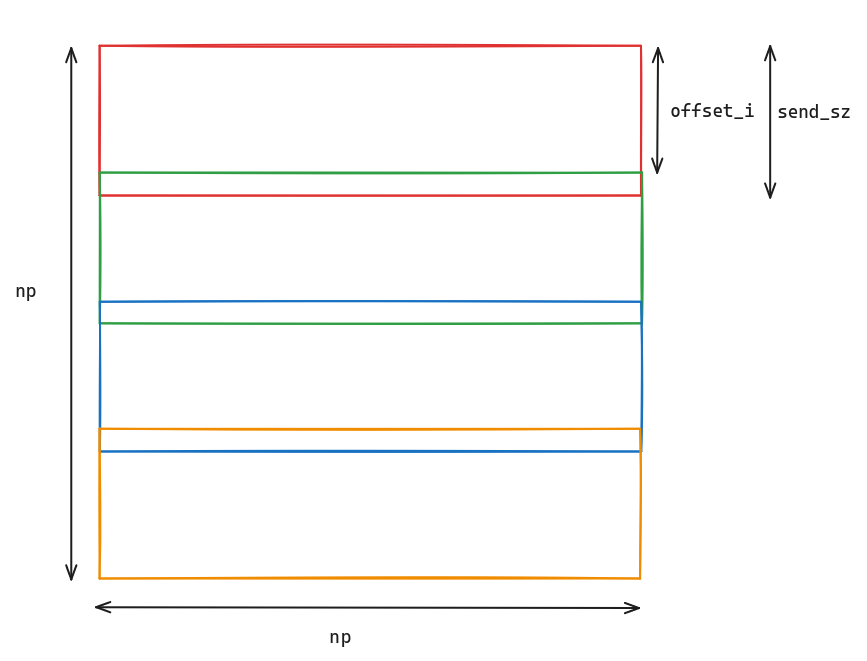
\includegraphics[width=1\textwidth]{mpi_jacobi_data_distribution.png}
\caption{Jacobi data distribution}
\label{fig:data_distribution}
\end{figure}

Upon receiving their respective initial data, the computation starts for each worker. Each process invokes \incode{relax_jacobi} on its local data, \incode{u} and \incode{uhelp}. Additionally, it sends its first internal row to the last halo row of the preceding process and its last internal row to the first halo row of the subsequent process, provided that these neighboring processes exist.

In order to check the convergence condition \incode{if (residual < 0.00005) break;}, each process calls \incode{MPI_Allresidual} to sum up all of the local residuals of each process and make the result visible to all of them, before checking the convergence condition.

Finally, the master process is in charge of gather all of the final local results of each worker process into its \incode{param.u matrix}, this is achieve with the last lines of code in both Code \ref{code:mpi_master} and \ref{code:mpi_workers}.

\begin{lstlisting}[label=code:mpi_master,style=c, language=C, caption=MPI Jacobi/Gauss-Seidel convergence for the master process, captionpos=b]
iter = 0;
while(1) {
    switch( param.algorithm ) {
        case 0: // JACOBI
            if (numprocs > 1){
                MPI_Recv(param.u+(rows+1)*np, np, MPI_DOUBLE, myid+1, 0, MPI_COMM_WORLD, MPI_STATUS_IGNORE);
                MPI_Send(param.u+rows*np, np, MPI_DOUBLE, myid+1, 0, MPI_COMM_WORLD);
            }

            residual = relax_jacobi(param.u, param.uhelp, rows + 2, np);

            memcpy(param.u, param.uhelp, sizeof(double)*(rows+2)*np);
            break;
        case 1: // GAUSS
            residual = relax_gauss(param.u, rows+2, np);
            if (myid < numprocs - 1){
                MPI_Recv(param.u+np*(rows+1), np, MPI_DOUBLE, myid+1, 0, 
                        MPI_COMM_WORLD, MPI_STATUS_IGNORE);
            }

            break;
    }

    iter++;
    MPI_Allreduce(MPI_IN_PLACE, &residual, 1, MPI_DOUBLE, MPI_SUM, MPI_COMM_WORLD);

    if (residual < 0.00005) break;
    if (param.maxiter>0 && iter>=param.maxiter) break;
}
int recv_sz = param.resolution/numprocs * np;

for (int id = 1; id < numprocs; id++){
    int offset = param.resolution/numprocs * np * id + np;
    MPI_Recv(param.u + offset, recv_sz, 
             MPI_DOUBLE, id, 0, MPI_COMM_WORLD, MPI_STATUS_IGNORE);
}
\end{lstlisting}

\begin{lstlisting}[label=code:mpi_workers,style=c, language=C, caption=MPI Jacobi/Gauss-Seidel convergence for the worker processes, captionpos=b]
iter = 0;
while(1) {
            switch( param.algorithm ) {
                case 0: // JACOBI
                if(numprocs > 1){
                    MPI_Recv(param.u+(rows+1)*np, np, MPI_DOUBLE, myid+1, 0, MPI_COMM_WORLD, MPI_STATUS_IGNORE);
                    MPI_Send(param.u+rows*np, np, MPI_DOUBLE, myid+1, 0, MPI_COMM_WORLD );
                }
                    residual = relax_jacobi(param.u, param.uhelp, rows + 2, np);
                    memcpy(param.u, param.uhelp, sizeof(double)*(rows+2)*np);
                    break;
                case 1: // GAUSS
                    residual = relax_gauss(param.u, rows+2, np);
                    if (myid < numprocs - 1){
                        MPI_Recv(param.u+np*(rows+1), np, MPI_DOUBLE, myid+1, 0, 
                                MPI_COMM_WORLD, MPI_STATUS_IGNORE);
                    }

                    break;
            }

            iter++;
            MPI_Allreduce(MPI_IN_PLACE, &residual, 1, MPI_DOUBLE, MPI_SUM, MPI_COMM_WORLD);

            if (residual < 0.00005) break;
            if (param.maxiter>0 && iter>=param.maxiter) break;
}
MPI_Send(u+np, rows*np, MPI_DOUBLE, 0, 0, MPI_COMM_WORLD);
\end{lstlisting}

The parallelization is illustrated visually in Figure \ref{fig:mpi_jacobi}

\begin{figure}[H]
\centering
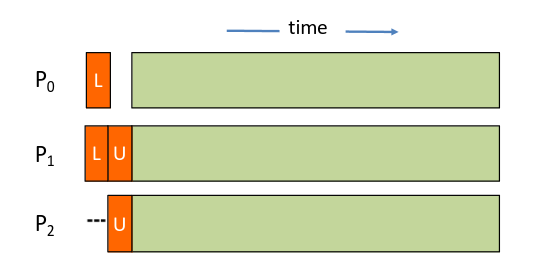
\includegraphics[width=0.7\textwidth]{mpi_jacobi.png}
\caption{MPI Jacobi parallelization}
\label{fig:mpi_jacobi}
\end{figure}

\subsubsection{Gauss-Seidel}
\label{sec:mpi_gauss_seidel}

Due to the dependencies present in the Gauss-Seidel method, it is not an \textit{embarrassing parallel} algorithm like the Jacobi parallelization. However, if we make the synchronization of rows between processes at a subcolumn (tile) level, we can exploit \textit{wavefront parallelism}

The difference between tiled and ``untiled" Gauss-Seidel parallelization is illustrated in Figure \ref{fig:mpi_gauss} and \ref{fig:mpi_gauss_tiled}.

\begin{figure}[H]
\centering
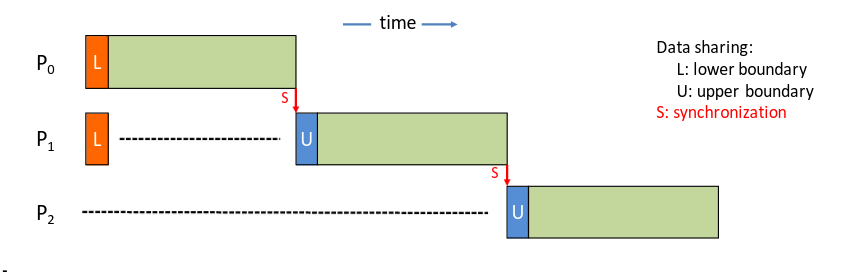
\includegraphics[width=1\textwidth]{mpi_gauss_normal.png}
\caption{MPI Gauss-Seidel parallelization without tiling}
\label{fig:mpi_gauss}
\end{figure}

\begin{figure}[H]
\centering
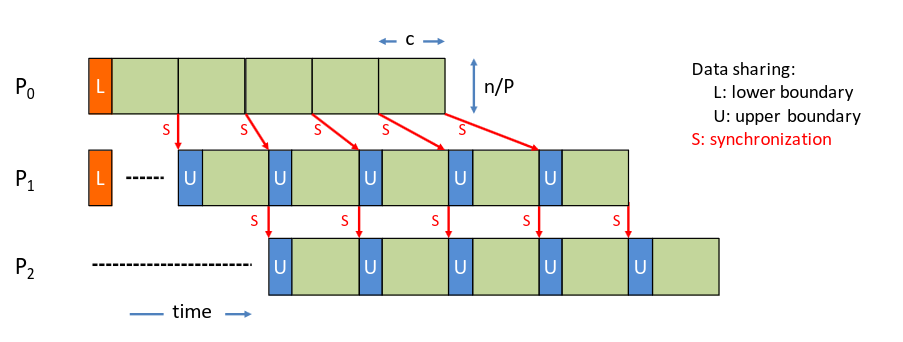
\includegraphics[width=1\textwidth]{mpi_gauss_tiled.png}
\caption{MPI Gauss-Seidel parallelization with tiling}
\label{fig:mpi_gauss_tiled}
\end{figure}

For the Gauss-Seidel parallelization, we have to modify the \incode{relax_gauss} function as shown in Code \ref{code:mpi_relax_gauss}. Notice how we perform de previous process' inner last row and next process' first halo row data synchornization at the tile level, to exploit, as we mentioned before, \textit{wavefront parallelism}. Finally, the only data synchronization is next process' first inner row to previous process' last halo row, which is accomplished in with the \incode{MPI_Recv} and \incode{MPI_Send} functions in Code \ref{code:mpi_master} and \ref{code:mpi_workers}

\begin{lstlisting}[label=code:mpi_relax_gauss,style=c, language=C, caption=MPI \incode{relax_gauss} function, captionpos=b]
double relax_gauss (double *u, unsigned sizex, unsigned sizey)
{
    double unew, diff, sum=0.0;
    int nby, by, numprocs;
    int rank;
    MPI_Comm_rank(MPI_COMM_WORLD, &rank);
    MPI_Request r;

    by = sizex - 2;
    nby = (sizey-2) / by;
    numprocs = nby;

    for (int jj = 0; jj < nby ; jj++) {
        if (rank > 0){
            int offset = jj * by + 1;
            MPI_Recv(u + offset, by, MPI_DOUBLE, rank - 1, 0, 
                    MPI_COMM_WORLD, MPI_STATUS_IGNORE );
        }

        for (int i=1; i < sizex-1; i++) {
            for (int j=1+jj*by; j < (jj+1)*by + 1; j++) {
                unew= 0.25 * 
                      ( u[ i*sizey + (j-1) ]+  // left
                        u[ i*sizey + (j+1) ]+  // right
                        u[ (i-1) * sizey + j ]+  // top
                        u[ (i+1) * sizey + j ]); // bottom

                diff = unew - u[i*sizey+j];
                sum += diff * diff; 
                u[i*sizey+j]=unew;
            }
        }

        if (rank < numprocs - 1 ){
            int offset = (sizex - 2) * sizey +  jj * by + 1;
            MPI_Isend( u + offset, by, MPI_DOUBLE, rank + 1, 0, 
                    MPI_COMM_WORLD, &r);
        }
    }

    return sum;
}
\end{lstlisting}

\subsection{CUDA}

For the CUDA solver, we have multiple ways to approach the problem:

\begin{enumerate}
    \item Parallel stencil and serial residual computation.
    \item Parallel stencil and parallel residual computation.
\end{enumerate}

\subsubsection{Serial residual}

We'll start by delving into the first approach, primarily for its simplicity. In this method, we aim to determine the required number of threads to cover the entire iteration space, including the halo, thus simplifying the kernel.

To determine the grid and block dimensions, we employ the following code snippet:

\begin{lstlisting}[style=c, language=C, caption=Grid and block dimension calculation, captionpos=b]
// full size (param.resolution are only the inner points)
np = param.resolution + 2;

int Grid_Dim, Block_Dim;    // Grid and Block structure values
if (strcmp(argv[2], "-t")==0) {
    Block_Dim = atoi(argv[3]);
    Grid_Dim = np/Block_Dim + ((np%Block_Dim)!=0);
    if ((Block_Dim*Block_Dim) > 512) {
        printf("Error -- too many threads in block, try again\n");
        return 1;
    }
}
dim3 Grid(Grid_Dim, Grid_Dim);
dim3 Block(Block_Dim, Block_Dim);
\end{lstlisting}

This results in:

\begin{itemize}
    \item The number of threads per block in each dimension being 8.
    \item The number of blocks per grid in each dimension being 33.
\end{itemize}

This yields a total of $8 \times 8 \times 33 \times 33 = 69696$ threads.

The overall CUDA solver process involves the following steps:

\begin{enumerate}
    \item Allocation of GPU memory for the \incode{u} and \incode{uhelp} matrices.
    \item Copying the current \incode{uhelp} and \incode{u} values from the host to the GPU.
    \item Executing the stencil computation for each element in the \incode{u} matrix by launching 69696 threads using the \incode{gpu_Heat} kernel while specifying the grid and block dimensions.
    \item The kernel handles the exclusion of values related to halo elements.
    \item Ensuring that all threads complete the kernel computation by invoking \incode{cudaDeviceSynchronize}.
    \item Calculating the residual on the host using values copied from the GPU for the \incode{u} and \incode{u_help} matrices.
    \item Repeating steps 3 to 6 as long as the computation has not converged and hasn't reached the maximum allowable iterations.
    \item Copying the results from the GPU back to the host.
    \item Freeing the GPU memory.
\end{enumerate}

\begin{lstlisting}[style=c, language=C, caption=CUDA code run in the Host, captionpos=b]
double *dev_u;
double *dev_uhelp;
double *dev_sum;

// TODO: Allocation on GPU for matrices u and uhelp
cudaMalloc(&dev_u, np*np*sizeof(double));
cudaMalloc(&dev_uhelp, np*np*sizeof(double));
cudaMalloc(&dev_sum, sizeof(double));

// TODO: Copy initial values in u and uhelp from host to GPU
cudaMemcpy(dev_u, param.u, np*np*sizeof(double), cudaMemcpyHostToDevice);
cudaMemcpy(dev_uhelp, param.uhelp, np*np*sizeof(double), cudaMemcpyHostToDevice);

iter = 0;
while(1) {
    gpu_Heat<<<Grid,Block>>>(dev_u, dev_uhelp, np);
    cudaDeviceSynchronize();  // Wait for compute device to finish.

    // TODO: residual is computed on host, we need to get from GPU values computed in u and uhelp
    cudaMemcpy(param.u, dev_u, np*np*sizeof(double), cudaMemcpyDeviceToHost);
    cudaMemcpy(param.uhelp, dev_uhelp, np*np*sizeof(double), cudaMemcpyDeviceToHost);

    residual = cpu_residual (param.u, param.uhelp, np, np);

    double * tmp = dev_u;
    dev_u = dev_uhelp;
    dev_uhelp = tmp;

    iter++;

    // solution good enough ?
    if (residual < 0.00005) break;

    // max. iteration reached ? (no limit with maxiter=0)
    if (iter>=param.maxiter) break;
}

// TODO: get result matrix from GPU
cudaMemcpy(param.u, dev_u, np*np*sizeof(double), cudaMemcpyDeviceToHost);

// TODO: free memory used in GPU
cudaFree(dev_u);
cudaFree(dev_uhelp);
\end{lstlisting}

\begin{lstlisting}[style=c, language=C, caption=CUDA kernel run in the device, captionpos=b]
#include <math.h>
#include <cuda.h>

__global__ void gpu_Heat(double *u, double *utmp, int N) {
    int sizey = N;
    int i = (blockIdx.y * blockDim.y) + threadIdx.y;
    int j = (blockIdx.x * blockDim.x) + threadIdx.x;

    if (i > 0 && i < N-1 && j > 0 && j < N-1){
        utmp[i*sizey+j]= 0.25 * (u[ i*sizey     + (j-1) ]+  // left
                u[ i*sizey     + (j+1) ]+  // right
                u[ (i-1)*sizey + j     ]+  // top
                u[ (i+1)*sizey + j     ]); // bottom
    }
}
\end{lstlisting}

This kernel calculates the row and column indices for each thread and incorporates an \incode{if} statement to exclude threads working on halo elements.

\subsubsection{Parallel residual}

For the reduction process, we've added several kernels to the \incode{kernels.cu} file, as depicted below:

\begin{lstlisting}[style=c, language=C, caption=CUDA kernel with reduction, captionpos=b]
#include <math.h>
#include <cuda.h>

__global__ void gpu_Diff(double *u, double *utmp, double* diffs, int N) {
    int i = (blockIdx.y * blockDim.y) + threadIdx.y;
    int j = (blockIdx.x * blockDim.x) + threadIdx.x;

    if (i > 0 && i < N-1 && j > 0 && j < N-1){
        utmp[i*N+j]= 0.25 * (u[ i*N     + (j-1) ]+  // left
                u[ i*N     + (j+1) ]+  // right
                u[ (i-1)*N + j     ]+  // top
                u[ (i+1)*N + j     ]); // bottom
        diffs[(i-1)*(N-2)+j-1] = (utmp[i*N+j] - u[i*N+j])*(utmp[i*N+j] - u[i*N+j]);
    }
}

__global__ void gpu_Heat_reduction(double *idata, double *odata, int N) {
        extern __shared__ double sdata[];
        unsigned int s;

        unsigned int tid = threadIdx.x;
        unsigned int i = blockIdx.x * (blockDim.x * 2) + threadIdx.x;
        unsigned int gridSize = blockDim.x * 2 * gridDim.x;
        sdata[tid] = 0;
        while (i < N) {
                sdata[tid] += idata[i] + idata[i + blockDim.x];
                i += gridSize;
        }
        __syncthreads();

        for (s = blockDim.x / 2; s > 32; s >>= 1) {
                if (tid < s)
                        sdata[tid] += sdata[tid + s];
                __syncthreads();
        }
        if (tid < 32) {
                volatile double *smem = sdata;

                smem[tid] += smem[tid + 32];
                smem[tid] += smem[tid + 16];
                smem[tid] += smem[tid + 8];
                smem[tid] += smem[tid + 4];
                smem[tid] += smem[tid + 2];
                smem[tid] += smem[tid + 1];
        }
        
        if (tid == 0)
                odata[blockIdx.x] = sdata[0];
}
\end{lstlisting}

Here, a new kernel, \incode{gpu_Diff}, has been introduced to enable each thread to execute the 2D stencil computation and store the squared result in the \incode{diffs} vector. Additionally, a kernel named \incode{gpu_Heat_reduction} has been added, directly sourced from Boada, to handle the reduction process, notice that we changed slightly the line of shared memory declaration, and we provide the explanation later in the report. This kernel is designed to compute the residual value on the GPU, utilizing shared memory per thread block.

\begin{lstlisting}[style=c, language=C, caption=Modified heat-CUDA.c, captionpos=b]
int main( int argc, char *argv[] ) {

    ...
    
    #define REDUCTION 1

    ...
    
    __global__ void gpu_Heat (double *h, double *g, int N);
    __global__ void gpu_Diff (double *h, double *g, double *diff, int N);
    __global__ void gpu_Heat_reduction (double *h, double *g, int N);


    ...
    
    double *dev_u;
    double *dev_uhelp;
    double *dev_diffs;
    double *dev_red1;
    double *dev_red2;

    const int MAX_THREADS_PER_BLK = 1024;
    int blocks = Grid_Dim * Grid_Dim; 
    int threads = Block_Dim * Block_Dim; 
    if (REDUCTION && blocks > MAX_THREADS_PER_BLK){
        threads = MAX_THREADS_PER_BLK;
        blocks = ((np-2) * (np-2) / threads) + ((np-2) * (np-2) % threads != 0);
    }

    // TODO: Allocation on GPU for matrices u and uhelp
    cudaMalloc(&dev_u, np*np*sizeof(double));
    cudaMalloc(&dev_uhelp, np*np*sizeof(double));
    if (REDUCTION){
        cudaMalloc(&dev_diffs, (np-2)*(np-2)*sizeof(double));
        cudaMalloc(&dev_red1, threads*sizeof(double));
        cudaMalloc(&dev_red2, blocks*sizeof(double));
    }

    // TODO: Copy initial values in u and uhelp from host to GPU
    cudaMemcpy(dev_u, param.u, np*np*sizeof(double), cudaMemcpyHostToDevice);
    cudaMemcpy(dev_uhelp, param.uhelp, np*np*sizeof(double), cudaMemcpyHostToDevice);
        double *res;
    if (REDUCTION)
        res = (double*)malloc(sizeof(double)*blocks);
    iter = 0;
    while(1) {
        if (REDUCTION){
            gpu_Diff<<<Grid, Block>>>(dev_u, dev_uhelp, dev_diffs, np);
            gpu_Heat_reduction<<<blocks, threads, threads*sizeof(double)>>>(dev_diffs, dev_red1, (np-2) * (np-2));
            gpu_Heat_reduction<<<1, blocks, blocks*sizeof(double)>>>(dev_red1, dev_red2, blocks);
            cudaDeviceSynchronize();  // Wait for compute device to finish.
            cudaMemcpy(res, dev_red2, sizeof(double)*blocks, cudaMemcpyDeviceToHost);
            residual = res[0];
        }else{
            gpu_Heat<<<Grid, Block>>>(dev_u, dev_uhelp, np);
            cudaDeviceSynchronize();  // Wait for compute device to finish.
            cudaMemcpy(param.u, dev_u, np*np*sizeof(double), cudaMemcpyDeviceToHost);
            cudaMemcpy(param.uhelp, dev_uhelp, np*np*sizeof(double), cudaMemcpyDeviceToHost);
            residual = cpu_residual (param.u, param.uhelp, np, np);
        }

        cudaMemcpy(dev_u, dev_uhelp, np*np*sizeof(double), cudaMemcpyHostToHost);

        iter++;
        // solution good enough ?
        if (residual < 0.00005) break;
        // max. iteration reached ? (no limit with maxiter=0)
        if (iter>=param.maxiter) break;
    }

    // TODO: get result matrix from GPU
    cudaMemcpy(param.u, dev_u, np*np*sizeof(double), cudaMemcpyDeviceToHost);

    // TODO: free memory used in GPU
    cudaFree(dev_u);
    cudaFree(dev_uhelp);
    cudaFree(dev_diffs);
    cudaFree(dev_red1);
    cudaFree(dev_red2);
    
    ...
}
\end{lstlisting}

Please note that to avoid saturating the report, we have displayed only the relevant segment of the code in \incode{heat-CUDA.cu}. 

In this updated version, the approach closely resembles the previous serial code, incorporating the following modifications:

\begin{enumerate}
    \item Definition of the \href{https://gcc.gnu.org/onlinedocs/cpp/Object-like-Macros.html}{object-like macro} \incode{REDUCTION} indicating whether to compute the \incode{residual} value using the CPU (0) or the GPU (1).
    \item Addition of two function prototypes, \incode{gpu_Diff} and \incode{gpu_Heat_reduction}, implemented as kernels in \incode{kernels.cu}.
    \item Invocation of \incode{gpu_Diff} instead of \incode{gpu_Heat} to modify the \incode{uhelp} matrix and calculate the square of differences, storing the result in the parameter \incode{diffs} which is a 1D vector.
    \item Utilization of shared memory for reduction, requiring two successive calls to \incode{gpu_Heat_reduction}. The first call aggregates the summed values of differences from multiple blocks, while the subsequent call computes the final scalar value of the residual.
    \item Adjustment of the number of threads per block in CUDA to limit the count of blocks per grid. This adjustment allows passing the number of blocks from the initial reduction kernel call to the subsequent call as the number of threads per block. This adaptation is necessary as the default value of 64 threads per block could potentially exceed the 1024-thread limit in the second kernel call if the number of blocks surpasses this limit.
    \item Furthermore, we specify a third argument in the kernel call's triple angle brackets (\incode{<<<...>>>}) to designate the length of the shared memory within each block. This feature is referred to as \href{https://developer.nvidia.com/blog/using-shared-memory-cuda-cc/}{Dynamic shared memory}. Enabling this functionality also requires the addition of the keyword \incode{extern} to the shared memory \incode{sdata}.
\end{enumerate}

\q{Complete a table or draw a plot in which you show the execution time and speedup (from 1, 2, 4 and 8 processors, with respect to the serial execution time) for the OpenMP and MPI parallel versions that you have developped. Indicate clearly the solver being used and the problem size.}

\subsection{Sequential results}

\begin{table}[H]
\begin{center}
    \begin{tabular}{ |c|c|c|c| } 
     \hline
     \bfseries{Algorithm} &
     \bfseries{256x256} &
     \bfseries{512x512} &
     \bfseries{1024x1024} 
     \\
     \hline
      Jacobi & 2.412 & 17.743 &  85.377 \\
      Gauss-Seidel & 4.531 & 39.916 &  167.666 \\
     \hline
    \end{tabular}
\end{center}
\caption{Sequential execution time in seconds}
\end{table}

\subsection{OpenMP results}

\begin{table}[H]
\begin{center}
    \begin{tabular}{ |c|c|c|c| } 
     \hline
     \bfseries{Threads} & \bfseries{Jacobi} &
     \bfseries{Gauss-Seidel w/doacross} &
     \bfseries{Gauss-Seidel w/task} \\
     \hline
     1 & 2.595 & 5.327 & 5.336 \\
     2 & 1.830 & 4.037 & 5.481 \\ 
     4 & 2.370 & 2.323 & 5.544 \\ 
     8 & 2.526 & 1.416 & 5.793 \\ 
     \hline
    \end{tabular}
\end{center}
\caption{Execution time in seconds with 256x256 resolution}
\end{table}
 
\begin{table}[H]
\begin{center}
    \begin{tabular}{ |c|c|c|c| } 
     \hline
     \bfseries{Threads} & \bfseries{Jacobi} &
     \bfseries{Gauss-Seidel w/doacross} &
     \bfseries{Gauss-Seidel w/task} \\
     \hline
     1 & 20.884 & 42.789 & 42.855 \\
     2 & 13.519 & 32.759 & 43.003 \\ 
     4 & 12.837 & 18.799 & 44.565 \\ 
     8 & 11.672 & 10.663 & 47.322 \\ 
     \hline
    \end{tabular}
\end{center}
\caption{Execution time in seconds with 512x512 resolution}
\end{table}


\begin{table}[H]
\begin{center}
    \begin{tabular}{ |c|c|c|c| } 
     \hline
     \bfseries{Threads} & \bfseries{Jacobi} &
     \bfseries{Gauss-Seidel w/doacross} &
     \bfseries{Gauss-Seidel w/task} \\
     \hline
     1 & 89.834 & 172.180 & 172.250 \\
     2 & 58.808 & 132.694 & 176.056 \\ 
     4 & 50.051 & 76.345 & 179.742 \\ 
     8 & 43.300 & 43.103 & 186.841 \\ 
     \hline
    \end{tabular}
\end{center}
\caption{Execution time in seconds with 1024x1024 resolution}
\end{table}

\begin{table}[H]
\begin{center}
    \begin{tabular}{ |c|c|c|c| } 
     \hline
     \bfseries{Threads} & \bfseries{Jacobi} &
     \bfseries{Gauss-Seidel w/doacross} &
     \bfseries{Gauss-Seidel w/task} \\
     \hline
     1 & 0.929 & 0.850 & 0.849 \\
     2 & 1.318 & 1.122 & 0.826 \\ 
     4 & 1.017 & 1.950 & 0.817 \\ 
     8 & 0.954 & 3,199 & 0.782 \\ 
     \hline
    \end{tabular}
\end{center}
\caption{Speedup with 256x256 resolution}
\end{table}
 
\begin{table}[H]
\begin{center}
    \begin{tabular}{ |c|c|c|c| } 
     \hline
     \bfseries{Threads} & \bfseries{Jacobi} &
     \bfseries{Gauss-Seidel w/doacross} &
     \bfseries{Gauss-Seidel w/task} \\
     \hline
     1 & 0.849 & 0,932 & 0.931 \\
     2 & 1.312 & 1,218 & 0.928 \\ 
     4 & 1,382 & 2,123 & 0,895 \\ 
     8 & 1,520 & 3.743 & 0,843 \\ 
     \hline
    \end{tabular}
\end{center}
\caption{Speedup with 512x512 resolution}
\end{table}


\begin{table}[H]
\begin{center}
    \begin{tabular}{ |c|c|c|c| } 
     \hline
     \bfseries{Threads} & \bfseries{Jacobi} &
     \bfseries{Gauss-Seidel w/doacross} &
     \bfseries{Gauss-Seidel w/task} \\
     \hline
     1 & 0,950 & 0.973 & 0.973 \\
     2 & 1,451 & 1.263 & 0.952 \\ 
     4 & 1.705 & 2.196 & 0.932 \\ 
     8 & 1,97 & 3.889 & 0.897 \\ 
     \hline
    \end{tabular}
\end{center}
\caption{Speedup with 1024x1024 resolution}
\end{table}

\subsection{MPI results}

As we can observe, with an increase in the number of threads, the execution slows down. This slowdown is a result of added overheads due to various threads requiring computed data from other threads, leading to wait times between them. Nevertheless, with an increase in the number of data elements (\incode{param.resolution}), better speedups are anticipated (known as \incode{weak scaling}).

We use ``-" for cases where the job got killed by \incode{Boada} due to time limit. 

\begin{table}[H]
\begin{center}
    \begin{tabular}{ |c|c|c| } 
     \hline
     \bfseries{Threads} & \bfseries{Jacobi} &
     \bfseries{Gauss-Seidel}\\
     \hline
     1 & 2.016  & 5.318 \\
     2 & 2.191 & 4.140 \\ 
     4 & 510.191 & 403.062 \\ 
     8 &  -  &  - \\ 
     \hline
    \end{tabular}
\end{center}
\caption{Execution time in seconds with 256x256 resolution}
\end{table}

\begin{table}[H]
\begin{center}
    \begin{tabular}{ |c|c|c| } 
     \hline
     \bfseries{Threads} & \bfseries{Jacobi} &
     \bfseries{Gauss-Seidel}\\
     \hline
     1 & 17.599  &  42.766 \\
     2 & 18.053 & 33.697 \\ 
     4 &  -  & -  \\ 
     8 &   - & -  \\ 
     \hline
    \end{tabular}
\end{center}
\caption{Execution time in seconds with 512x512 resolution}
\end{table}

\begin{table}[H]
\begin{center}
    \begin{tabular}{ |c|c|c| } 
     \hline
     \bfseries{Threads} & \bfseries{Jacobi} &
     \bfseries{Gauss-Seidel}\\
     \hline
     1 & 76.695 & 172.191 \\
     2 & 73.519 &  135.184\\ 
     4 & - & -  \\ 
     8 & - & -  \\ 
     \hline
    \end{tabular}
\end{center}
\caption{Execution time in seconds with 1024x1024 resolution}
\end{table}

\begin{table}[H]
\begin{center}
    \begin{tabular}{ |c|c|c| } 
     \hline
     \bfseries{Threads} & \bfseries{Jacobi} &
     \bfseries{Gauss-Seidel}\\
     \hline
     1 & 1.196 & 0.852  \\
     2 & 1.100 & 1.094  \\ 
     4 & 0.008 & 0.011 \\ 
     8 & - & -  \\ 
     \hline
    \end{tabular}
\end{center}
\caption{Speedup with 256x256 resolution}
\end{table}

\begin{table}[H]
\begin{center}
    \begin{tabular}{ |c|c|c| } 
     \hline
     \bfseries{Threads} & \bfseries{Jacobi} &
     \bfseries{Gauss-Seidel}\\
     \hline
     1 & 1.008 & 0.933  \\
     2 & 0.982 & 1.184 \\ 
     4 & - & -  \\ 
     8 & -  & -   \\ 
     \hline
    \end{tabular}
\end{center}
\caption{Speedup with 512x512 resolution}
\end{table}

\begin{table}[H]
\begin{center}
    \begin{tabular}{ |c|c|c| } 
     \hline
     \bfseries{Threads} & \bfseries{Jacobi} &
     \bfseries{Gauss-Seidel}\\
     \hline
     1 & 1.113 &  0.973 \\
     2 & 1.161 &  1.240 \\ 
     4 & -  &  -  \\ 
     8 & - & -  \\ 
     \hline
    \end{tabular}
\end{center}
\caption{Speedup with 1024x1024 resolution}
\end{table}

\q{Include the source codes with the OpenMP, MPI and CUDA parallelizations
of the heat equation application for the solvers that you have studied.}

The source codes are included in the tar.gz file.

\end{document}